\section{Topology Optimization Overview}
\begin{wrapfigure}{R}{0.45\textwidth}
\centering
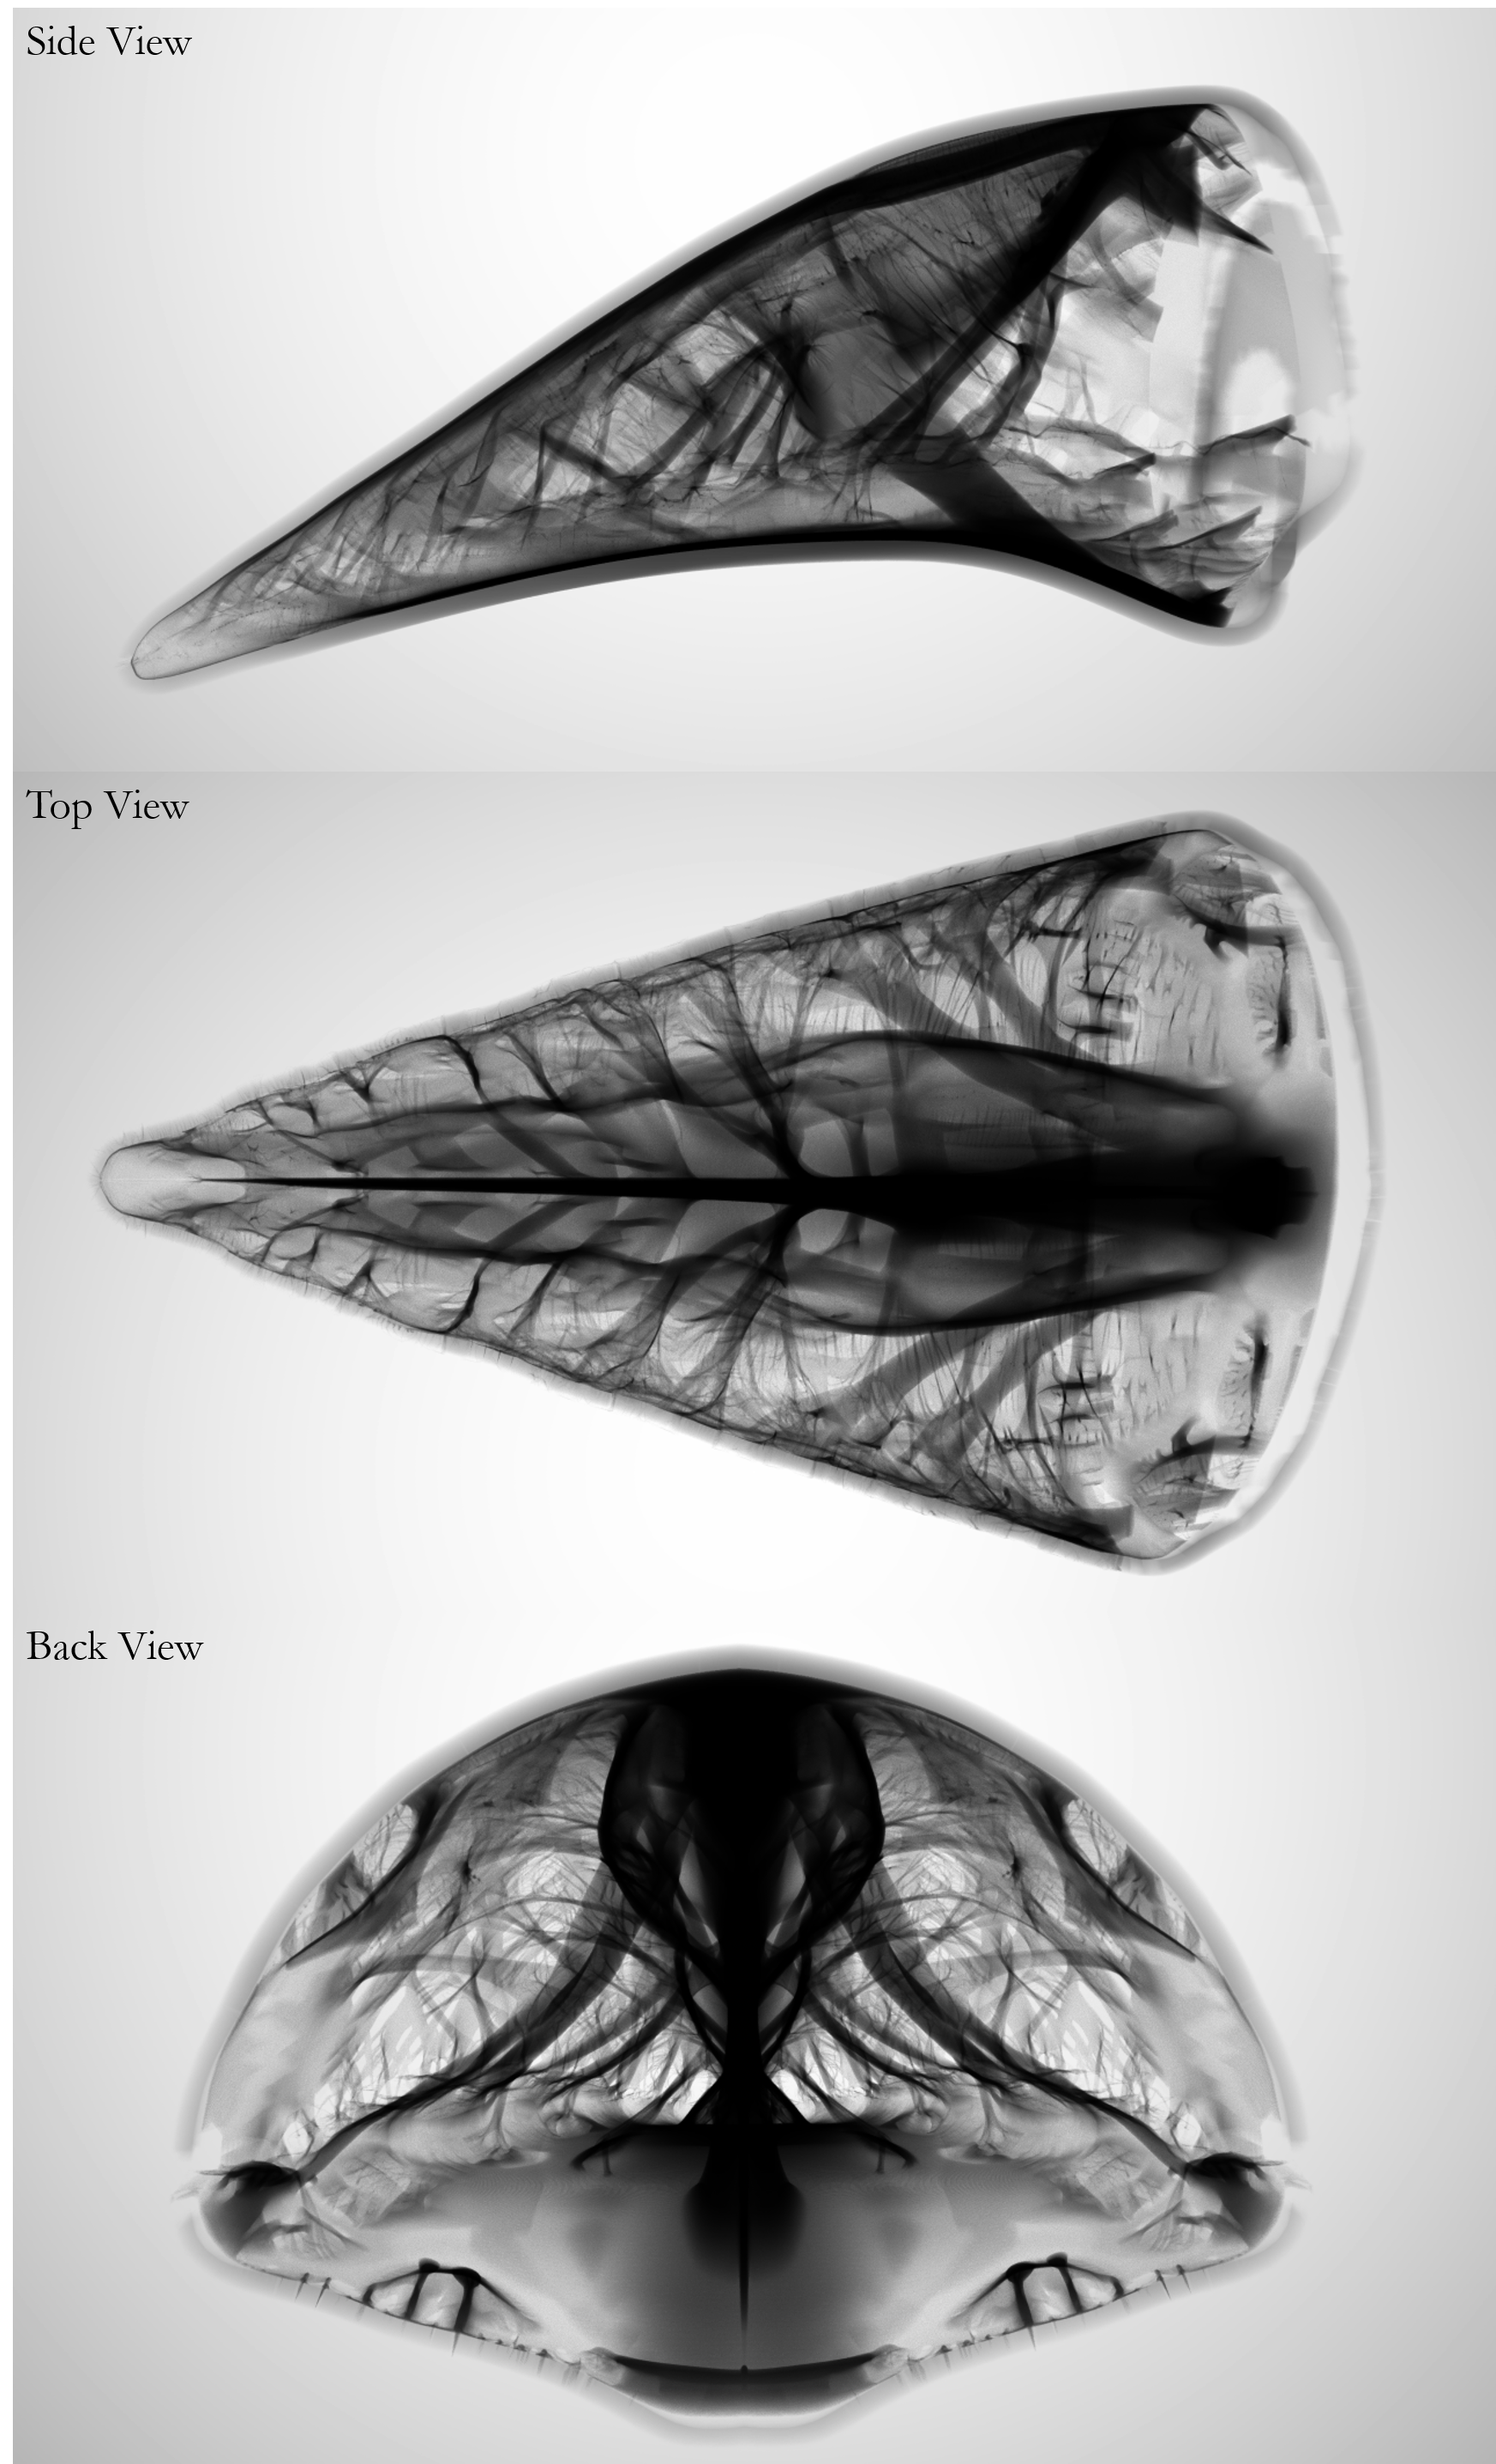
\includegraphics[width=0.42\textwidth]{images/TopOpt/beak_teaser}
\caption{The interior structures supporting the shell of a bird beak generated using our narrow-band topology optimization algorithm with $1,040,875,347$ (1.04 billion) active FEM voxels. The resolution of the background grid is $3000 \times 2400 \times 1600$. The three figures show the volumetric rendering of the same structure from different views.}
\label{fig:beak}
\end{wrapfigure}
Topology optimization aims to solve the problem of distributing materials in a given domain that minimizing the structural compliance or other objectives to given load(s).
It has demonstrated its efficacy in creating mechanical designs with complex structures and extreme properties in various engineering problems (see \cite{rozvany2009critical}, \cite{sigmund2013topology}, \cite{deaton2014survey} for surveys).
Starting from a volumetric domain that is uniformly filled with material, a standard topology optimization algorithm iteratively removes and redistributes material to develop a structure that minimizes a design objective (e.g., structural compliance), given the prescribed target volume and boundary conditions.  

However, due to the limitations of the previous computational frameworks, it is challenging to perform a standard topology optimization algorithm to emerge and evolve these thin and sparse features.
For example, to model the evolution of a thin sheet at the length scale of ten micrometers within a centimeter cube, it requires an FEM solver discretized on a $1000^3$ Cartesian grid. 
This grid resolution amounts to the order of magnitude of one billion active elements.

Recent advances in supercomputing provide some solutions that overcome this challenge.
For example, \cite{Aage2017GigavoxelCM} ran a parallel topology optimization program on a cluster with 8000 cores for days and obtained the structure of an airplane wing with the computational domain filled with 1.1 billion voxels.
A variety of novel, intricate, and multi-scale structures naturally emerge from the super-resolution computations.
This result is impressive, yet the limited accessibility and high cost of the supercomputing resources impede the use of such numerical approaches in a broader range of research and engineering applications. 
New computational tools, which are easy to access, efficient to run, and able to solve super-resolution systems, are needed in the scientific community.

\section{Main Contributions}
We propose a new computation framework that combines a sparse representation in conjunction with a highly optimized elastic multigrid solver for topology optimization, which delivers a significant leap in solving super-resolution problems from the prior state-of-the-art results.
Our framework has enabled the simulation of a sparsely populated computational domain on the level of billion active grid voxels on a single workstation. 
By examining the simulation results at such scale, we identify and analyze new challenges that have not been addressed, or even observed, in the previous research on elastic deformation simulation and topology optimization, such as poor asymptotic convergence of standard Galerkin-coarsened multigrid algorithm and the algorithmic limits of floating-point precision.

To address these scale-dependent challenges, we combined design practices and algorithmic interventions on data structures, numerical methods, and parallel solver implementations.
First, our framework is centered around a sparsely populated grid data structure, which allows the dynamic allocation of the degrees of freedom within a narrow band around the structure.  
This data structure combines the benefits of sparse storage, implicit topology representation, and the performance potential of high-throughput stream processing.
We have observed and demonstrated numerically that the elements with high structural sensitivities, which are essential for developing the structure towards its optimal topology, tend to bundle within a narrow band around the structure during evolution. 
In contrast, the vast bulk of void regions far from the structure contribute little to the total structural compliance, but they are the primary source of the computational cost in a dense discretization.
Therefore, the computation can be dramatically reduced by using a dynamically allocated sparse discretization, i.e the narrow-band representation.

In addition to the narrow-band representation, we developed a novel mixed-precision multigrid solver that is capable of solving FEM discretized linear elasticity in the order of billion elements on a single workstation.
By proposing an SPGrid-optimized matrix-free formulation for data storage and a novel mixed-precision computation, the solver can meet the memory storage and bandwidth demands of a multiprocessor workstation while maintaining high accuracy.
Also, our vectorized multigrid solver takes advantage of the AVX512 instruction set on the Intel Skylake-X/SP architecture in order to further enhance performance.

We summarize the main contributions of our work as follows:
\begin{itemize}
\item We demonstrate an ensemble of data structures, numerical schemes, and implementation best practices to perform topology optimization with the highest resolution (over one billion voxels) on a single shared-memory multiprocessor.
\item We propose a sparse, adaptive topology optimization framework where simulation of elastic deformation is restricted to a narrow band surrounding the high-density region.
\item We demonstrate the capacity of our framework to obtain a variety of complex thin and codimensional features, such as thin films and beams, that previous approaches might suppress.
\end{itemize}